\documentclass[a5paper,10pt,twoside]{book}

\usepackage[pass]{geometry}
\usepackage{blindtext}
\usepackage{fancyhdr}
\usepackage{graphicx}
\usepackage{titlesec}
\usepackage{wrapfig}
\usepackage[utf8]{inputenc}


% Make it A5.
\pdfpageheight=210mm
\pdfpagewidth=148mm
\addtolength{\textheight}{.875in}

% with this we ensure that the chapter and section
% headings are in lowercase.
\renewcommand{\chaptermark}[1]{\markboth{#1}{}}
\renewcommand{\sectionmark}[1]{\markright{\thesection\ #1}}
\fancyhf{}  % delete current header and footer
\fancyhead[LE,RO]{\bfseries\thepage}
\fancyhead[LO]{\bfseries\rightmark}
\fancyhead[RE]{\bfseries\leftmark}
\renewcommand{\headrulewidth}{0.5pt}
\renewcommand{\footrulewidth}{0pt}
\addtolength{\headheight}{0.5pt} % space for the rule
\fancypagestyle{plain}{%
   \fancyhead{} % get rid of headers on plain pages
   \renewcommand{\headrulewidth}{0pt} % and the line
}

% Remove numbers on empty pages.
\let\origdoublepage\cleardoublepage
\newcommand{\clearemptydoublepage}{%
  \clearpage
  {\pagestyle{empty}\origdoublepage}%
}
\let\cleardoublepage\clearemptydoublepage

\titleformat{\chapter}[display]{}{}{1ex}{\bfseries\LARGE}[]
\titlespacing{\chapter}{0pt}{-100pt}{40pt}

\begin{document}

\begin{titlepage}
\begin{center}

\includegraphics[width=10cm]{boi2014}\\[2cm]
{\bfseries\Huge Baltic Olympiad in Informatics}\\[1.5cm]
{\Huge\it Programme}\\
\vfill
{\bfseries\LARGE Palanga, 2014}
\end{center}
\end{titlepage}

\chapter{Foreword}

\begin{wrapfigure}[9]{r}{0.3\textwidth}
  \begin{center}
    \vspace{-20pt}
    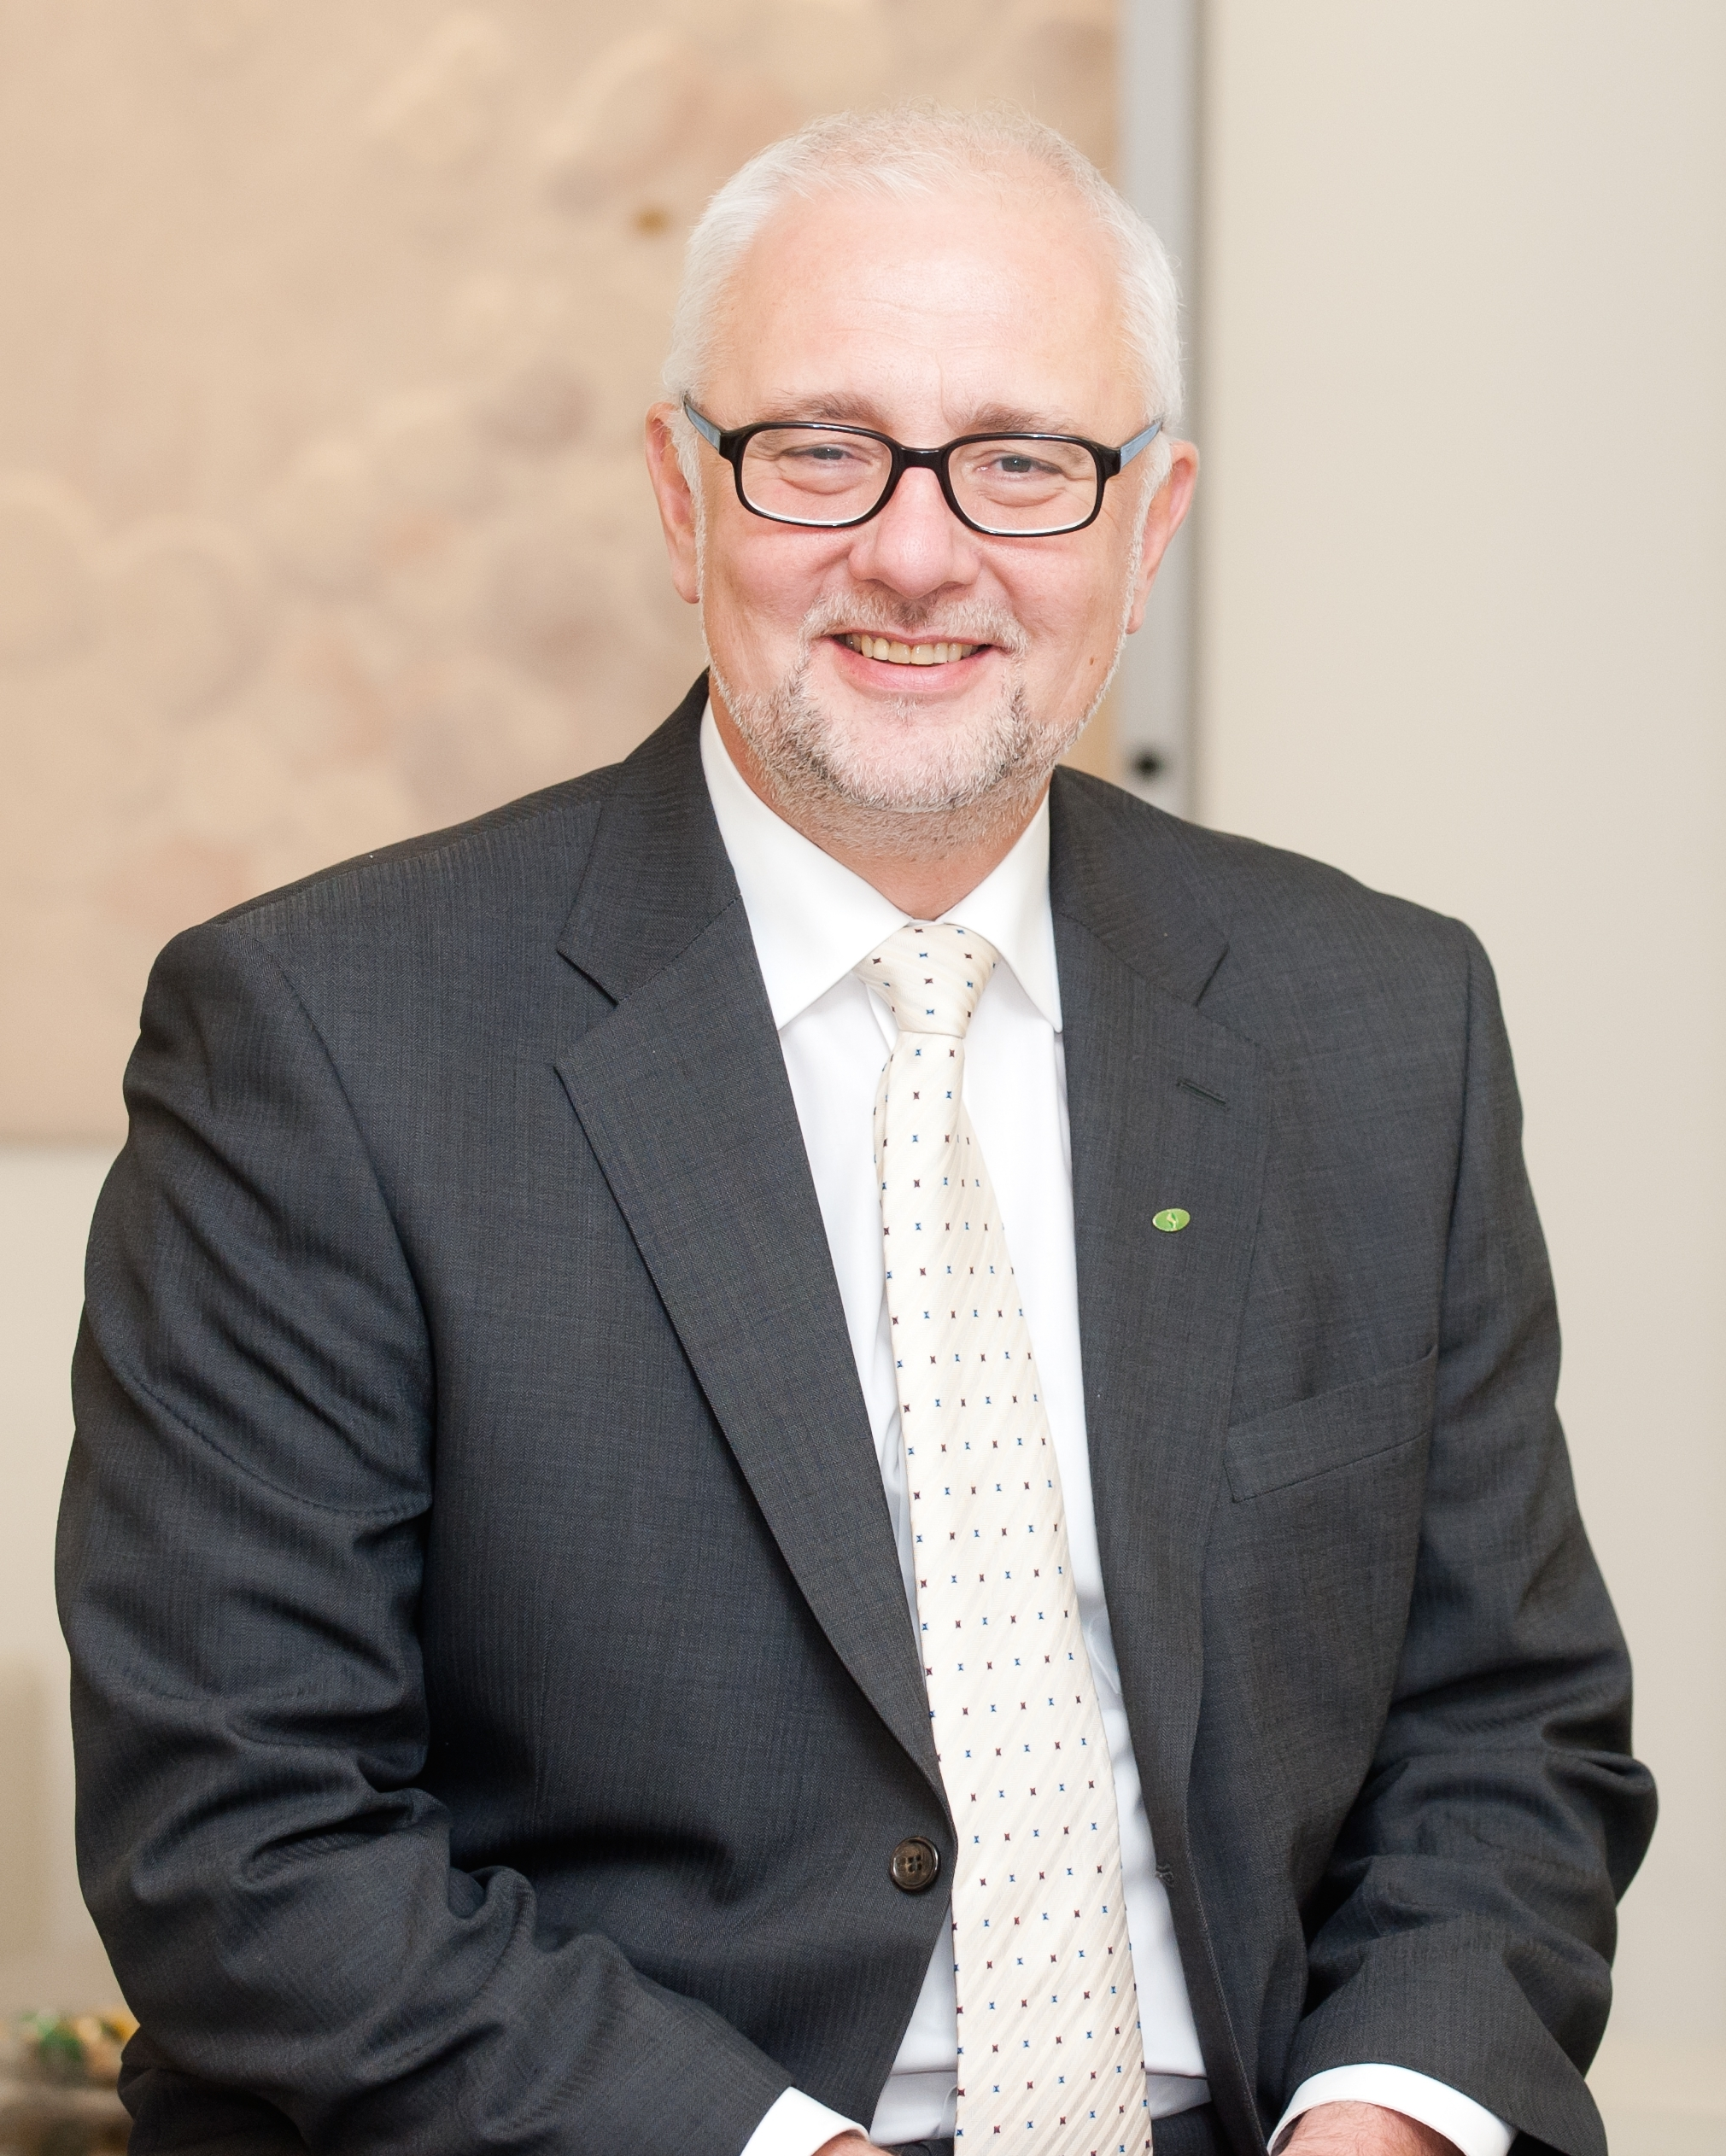
\includegraphics[width=0.28\textwidth]{ministras}
  \end{center}
\end{wrapfigure}
The 20th Baltic Olympiad in Informatics is celebrated in Lithuania with 60
participants from 9 countries situated around the Baltic Sea.

It is a joyful event for us with the most gifted young programmers as well as
the delegation leaders who are searching for, discovering and fostering pupils'
talent in the field of informatics science. We are especially glad that the
Olympiad is held at such a time when Europe is intensively seeking for
possibilities to promote teaching of informatics and computer science not only
in universities or colleges, but also in secondary schools and gymnasiums. There
is a lack of IT professionals able to grasp what lies behind technologies, able
to change them and innovative and smarter tools and technologies.

\blindtext

\blindtext

\blindtext

\chapter{Scientific Committee}

\setlength{\tabcolsep}{0.3cm}
\begin{tabular}{ c c c }
    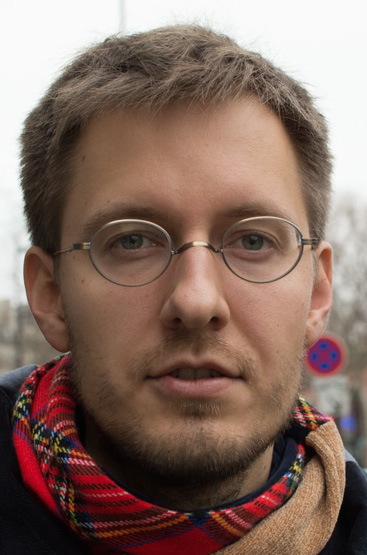
\includegraphics[width=2.5cm]{SC-LinasPetrauskas} &
    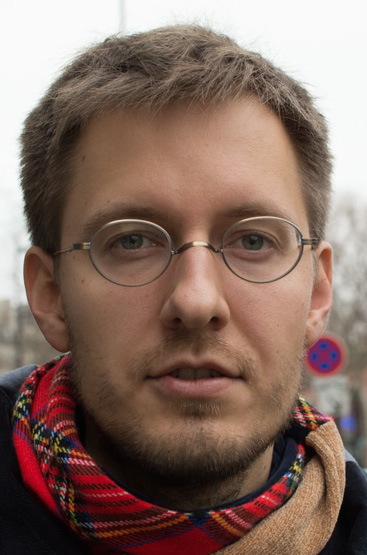
\includegraphics[width=2.5cm]{SC-LinasPetrauskas} &
    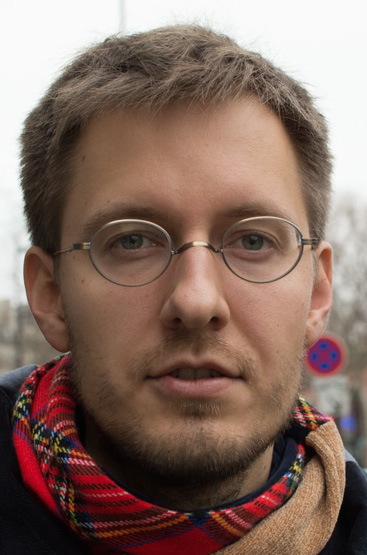
\includegraphics[width=2.5cm]{SC-LinasPetrauskas} \\
    Daumilas Ardickas &
    Donatas Kučinskas &
    Marijonas Petrauskas \\ [0.5cm]
    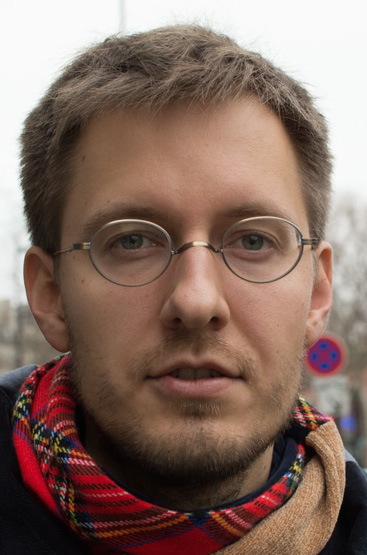
\includegraphics[width=2.5cm]{SC-LinasPetrauskas} &
    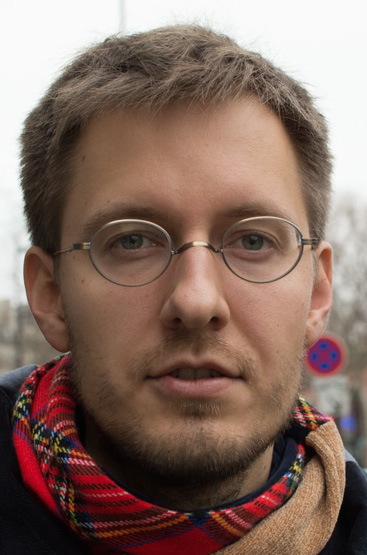
\includegraphics[width=2.5cm]{SC-LinasPetrauskas} &
    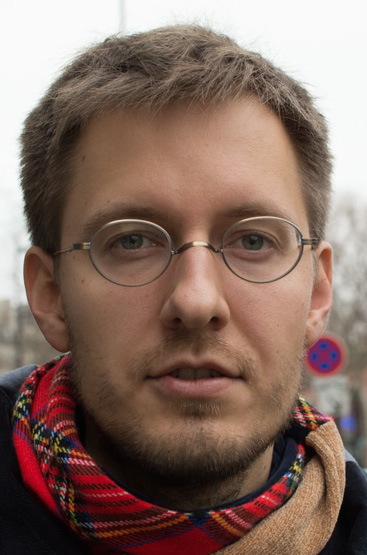
\includegraphics[width=2.5cm]{SC-LinasPetrauskas} \\
    Karolis Kusas &
    Kęstutis Vilčinskas &
    Vytautas Gruslys \\ [0.5cm]
    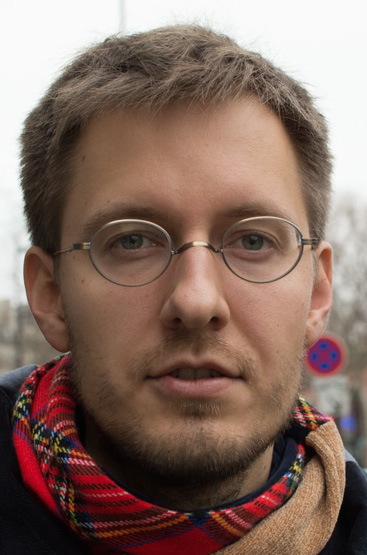
\includegraphics[width=2.5cm]{SC-LinasPetrauskas} \\
    Linas Petrauskas
\end{tabular}

\chapter{Schedule}

\setlength{\tabcolsep}{0.3cm}
\begin{tabular}{|c|c|c|}
    \hline
    {\bf Time} & {\bf Contestants} & {\bf Team Leaders} \\
    \hline
    Before 14:00 &
    \multicolumn{2}{|c|}{
        \begin{tabular}[x]{@{}c@{}}Arrival\\{\it Neringa}\end{tabular}
    } \\
    \hline
\end{tabular}

\end{document}
